\chapter{Этапы подготовки и анализа данных} \label{ch2}

В этой главе описываются этапы расширения и унификации экспериментальных данных, необходимых для обучения моделей. В параграфе \ref{ch2:augment} исходные таблицы аугментируются с сохранением исходных статистических свойств. Затем в параграфе \ref{ch2:proccessed} они объединяются в единый набор, и после анализа пропусков формируются три итоговые версии датасета: для CatBoost, для других ансамблевых методов (XGBoost, RF, GBR) и для MLR и SVR.

\section{Аугментация экспериментальных данных} \label{ch2:augment}

Для повышения обобщающей способности прогнозных моделей и расширения пространства признаков, доступных на этапе обучения, была проведена аугментация исходных данных. Основной целью процедуры являлось создание дополнительных наблюдений, сохраняющих ключевые статистические характеристики целевых переменных, но варьирующих параметры в пределах допустимого диапазона. Такой подход особенно оправдан при ограниченном объёме эмпирических данных, полученных из публикаций, где количество наблюдений зачастую невелико, а разнообразие условий проведения экспериментов недостаточно для обучения устойчивых моделей машинного обучения \cite{Shorten2019, Feng2021}.

Аугментация выполнялась отдельно для каждого датасета, после чего формировались два дополнительных набора: с увеличением объёма данных в пять и в десять раз по сравнению с оригинальным. Варьирование признаков осуществлялось при помощи стохастического отклонения значений отдельных параметров (например, морфологических характеристик растения, метеоусловий, высоты полёта и скорости обработки) в пределах заранее заданных границ. Они определялись либо на основе допусков, зафиксированных в первоисточниках \cite{Liu2025, Wu2025, Vitoria2022}, либо на предварительном анализе разброса по исходным данным. Для различных признаков варьирование осуществлялось с разной интенсивностью, например, параметры метеоусловий и опрыскивания допускали большую степень отклонения, чем морфологические признаки растений.

Для валидации корректности применённой процедуры аугментации были построены сравнительные графики целевых метрик --- покрытия поверхности растения рабочей жидкостью (coverage, в \%) и среднего диаметра капель (droplet size, в мкм). На \firef{fig:augment-coverage} и \firef{fig:augment-droplet-size} представлены результаты для оригинальных и аугментированных выборок (с коэффициентами увеличения ×5 и ×10), рассчитанные отдельно для каждого из экспериментальных источников: AGRAS T30 и T40 по данным \cite{Wu2025}, AGRAS T20 по \cite{Liu2025}, JT5L-404 по \cite{Vitoria2022}.

\begin{figure}[htbp]
	\begin{minipage}{0.95\linewidth}
	\adjustbox{minipage=1.3em,valign=t}{\subcaption{}\label{fig:augcov-a}}%
	\begin{subfigure}[t]{\dimexpr.5\linewidth-1.3em\relax}
		\centering
		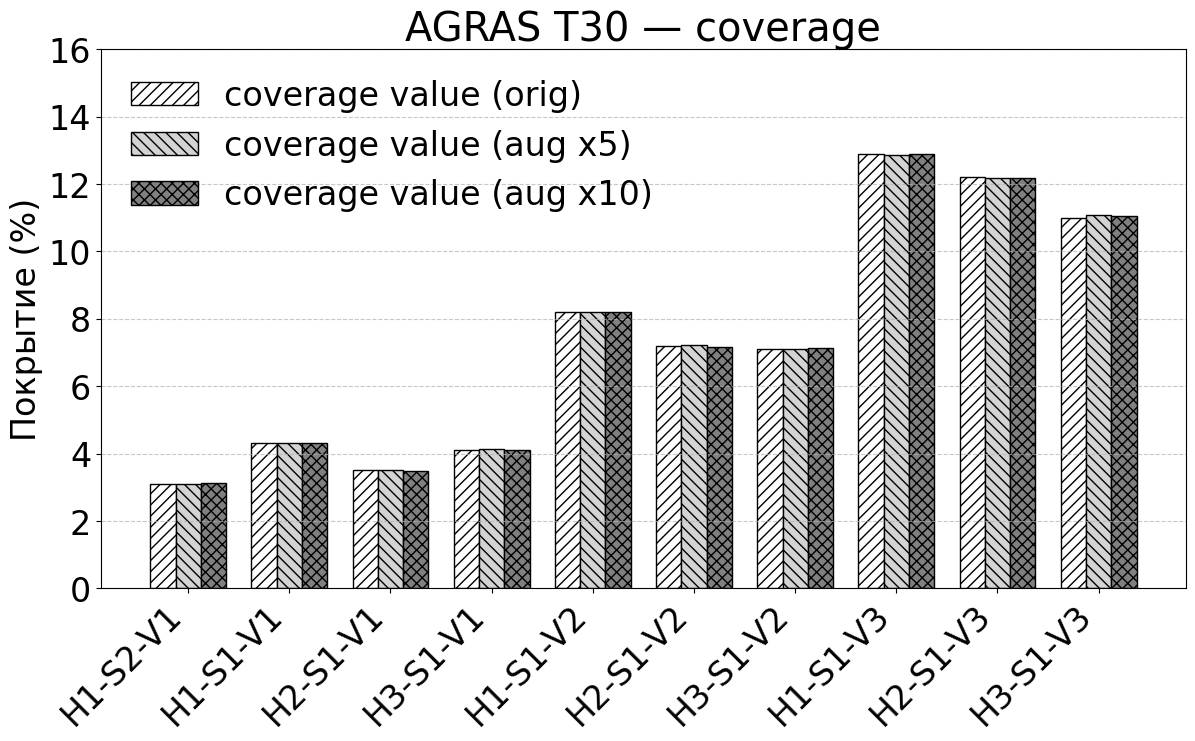
\includegraphics[width=.95\linewidth,valign=t]{my_folder/images/augment/spraying_performance/T30-coverage.png}
	\end{subfigure}
	\hfill %выровнять по ширине
		\adjustbox{minipage=1.3em,valign=t}{\subcaption{}\label{fig:augcov-b}}%
		\begin{subfigure}[t]{\dimexpr.5\linewidth-1.3em\relax}
			\centering
			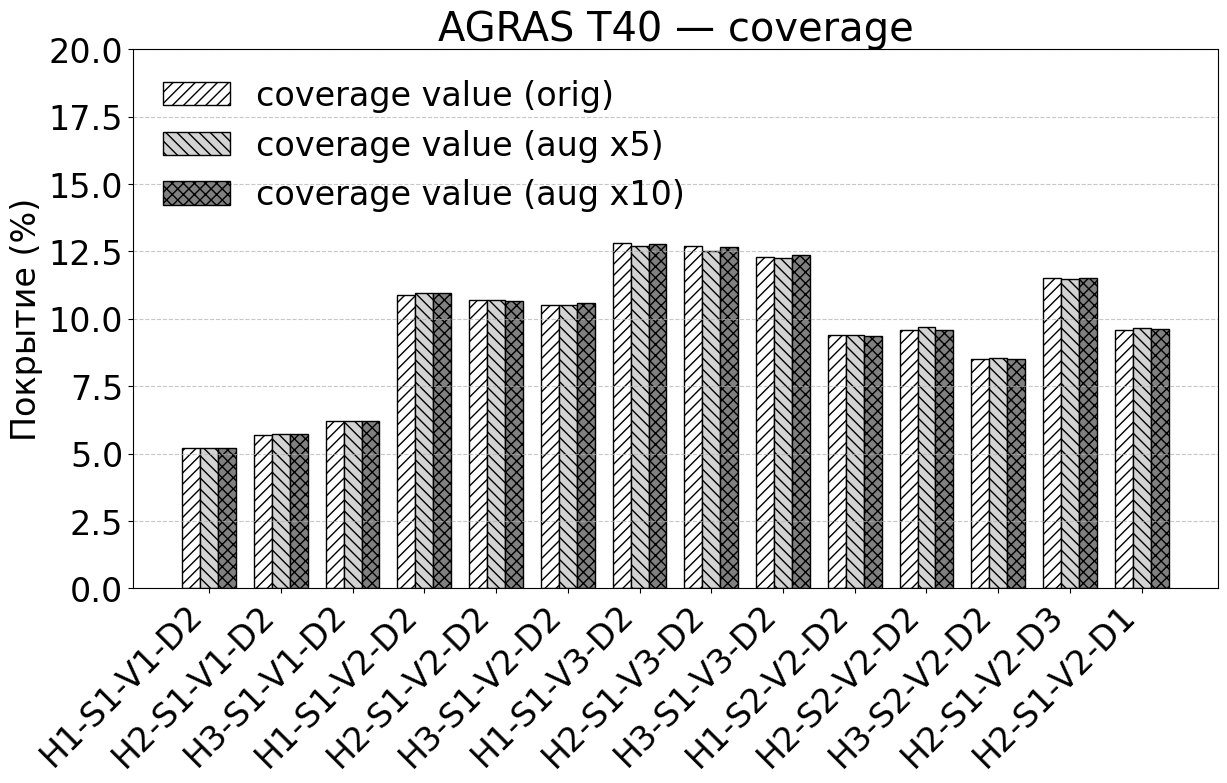
\includegraphics[width=.95\linewidth,valign=t]{my_folder/images/augment/spraying_performance/T40-coverage.png}
		\end{subfigure}
	\\[20pt]
		\adjustbox{minipage=1.3em,valign=t}{\subcaption{}\label{fig:augcov-c}}%
	\begin{subfigure}[t]{\dimexpr.5\linewidth-1.3em\relax}
		\centering
		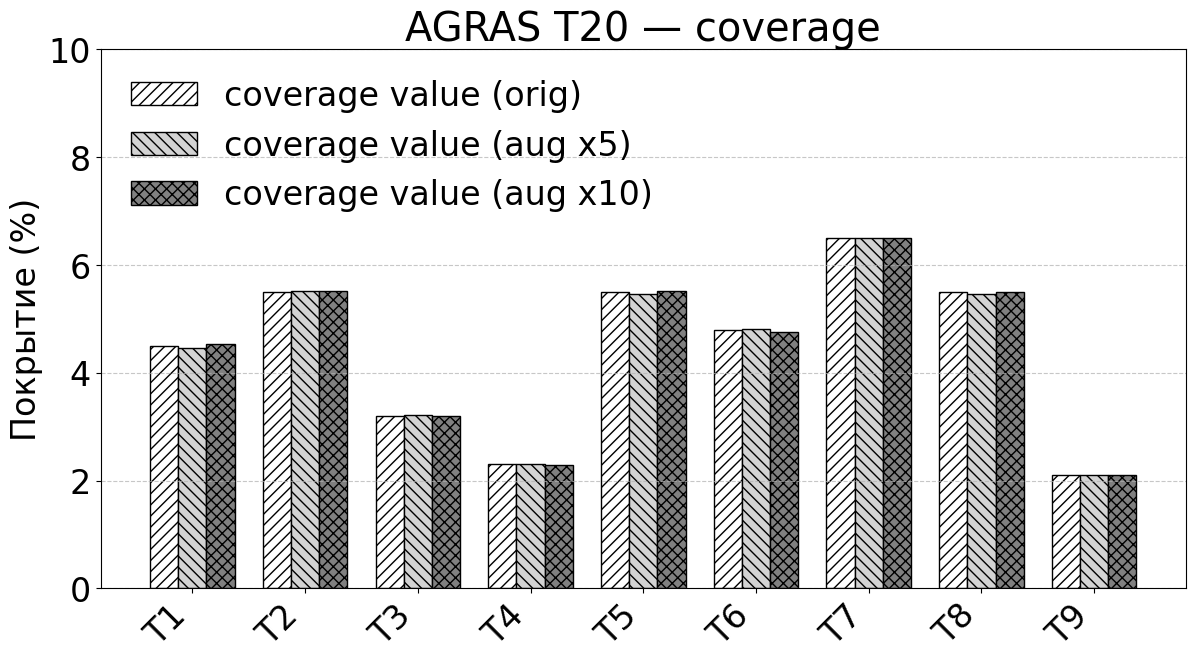
\includegraphics[width=.95\linewidth,valign=t]{my_folder/images/augment/droplet_deposition/T20-coverage.png}
	\end{subfigure}%
	\hfill %выровнять по ширине
	\adjustbox{minipage=1.3em,valign=t}{\subcaption{}\label{fig:augcov-d}}%
	\begin{subfigure}[t]{\dimexpr.5\linewidth-1.3em\relax}
		\centering
		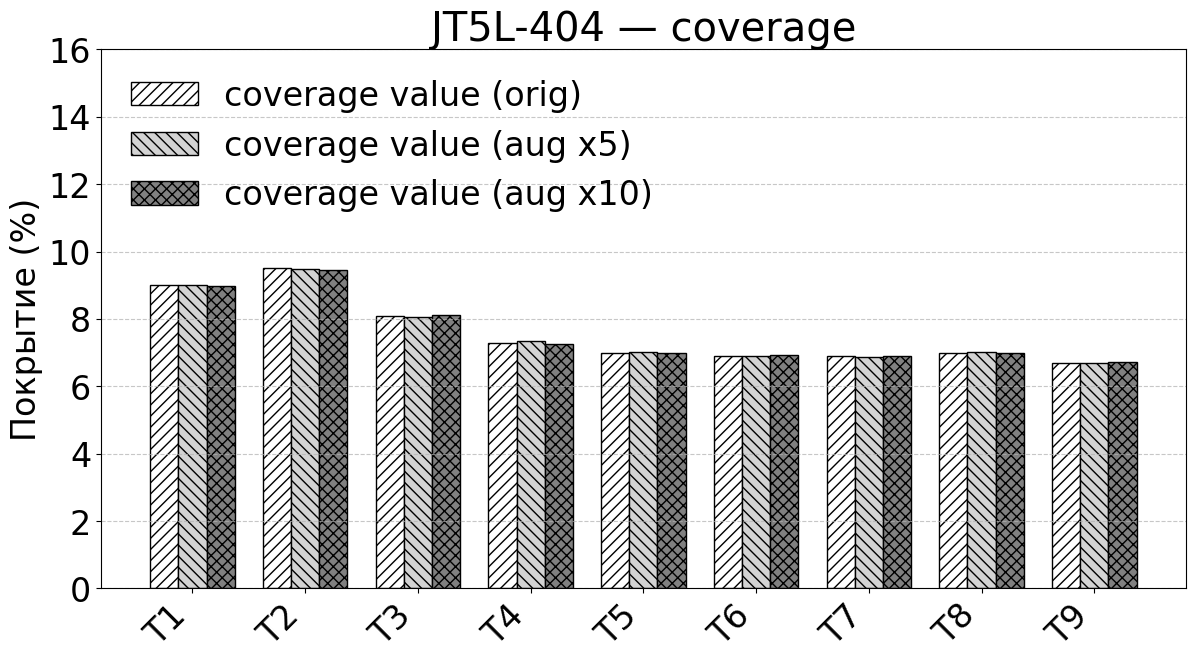
\includegraphics[width=.95\linewidth,valign=t]{my_folder/images/augment/coffee_science/JT5-coverage.png}
	\end{subfigure}
	\end{minipage}
	\captionsetup{justification=centering} %центрировать
	\caption{Распределение значений процента покрытия в исходной и аугментированных выборках: {\itshape a} --- AGRAS T30; {\itshape b} --- AGRAS T40; {\itshape c} --- AGRAS T20; {\itshape d} --- JT5L-404} 
	\label{fig:augment-coverage}
\end{figure}

\begin{figure}[htbp]
	\begin{minipage}{0.95\linewidth}
	\adjustbox{minipage=1.3em,valign=t}{\subcaption{}\label{fig:augds-a}}%
	\begin{subfigure}[t]{\dimexpr.5\linewidth-1.3em\relax}
		\centering
		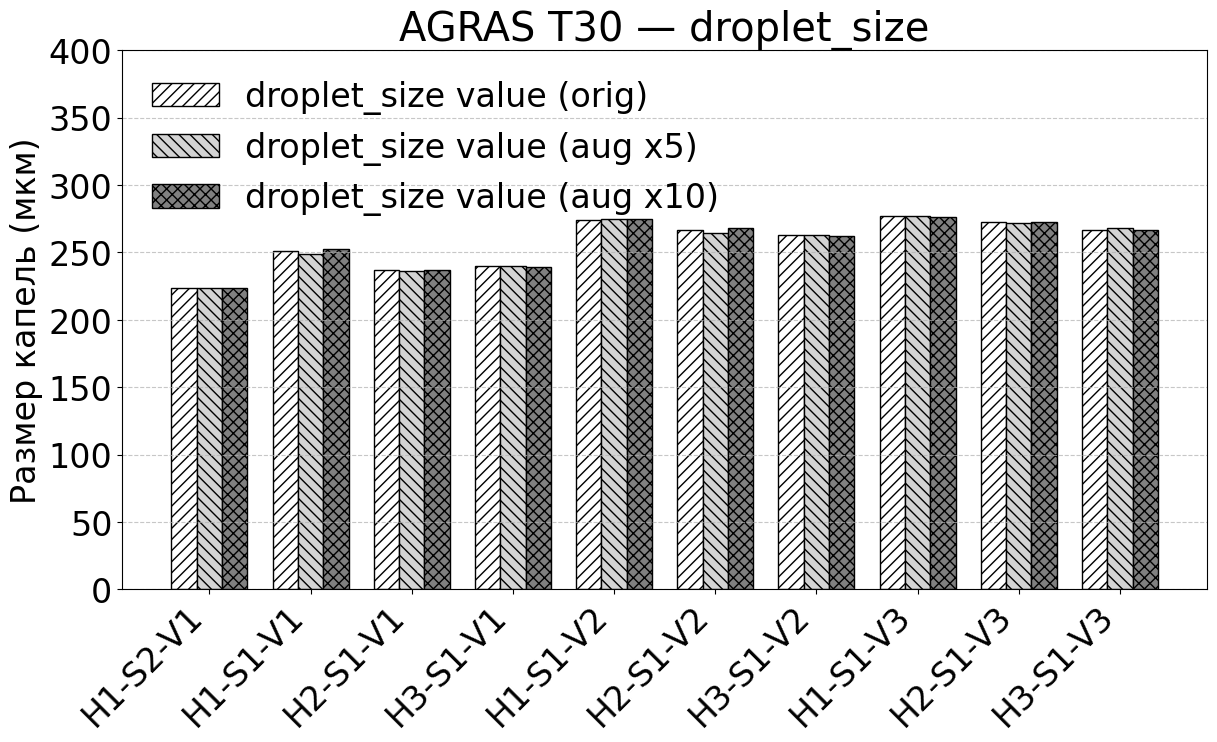
\includegraphics[width=.95\linewidth,valign=t]{my_folder/images/augment/spraying_performance/T30-droplet-size.png}
	\end{subfigure}
	\hfill %выровнять по ширине
	\adjustbox{minipage=1.3em,valign=t}{\subcaption{}\label{fig:augds-b}}%
	\begin{subfigure}[t]{\dimexpr.5\linewidth-1.3em\relax}
		\centering
		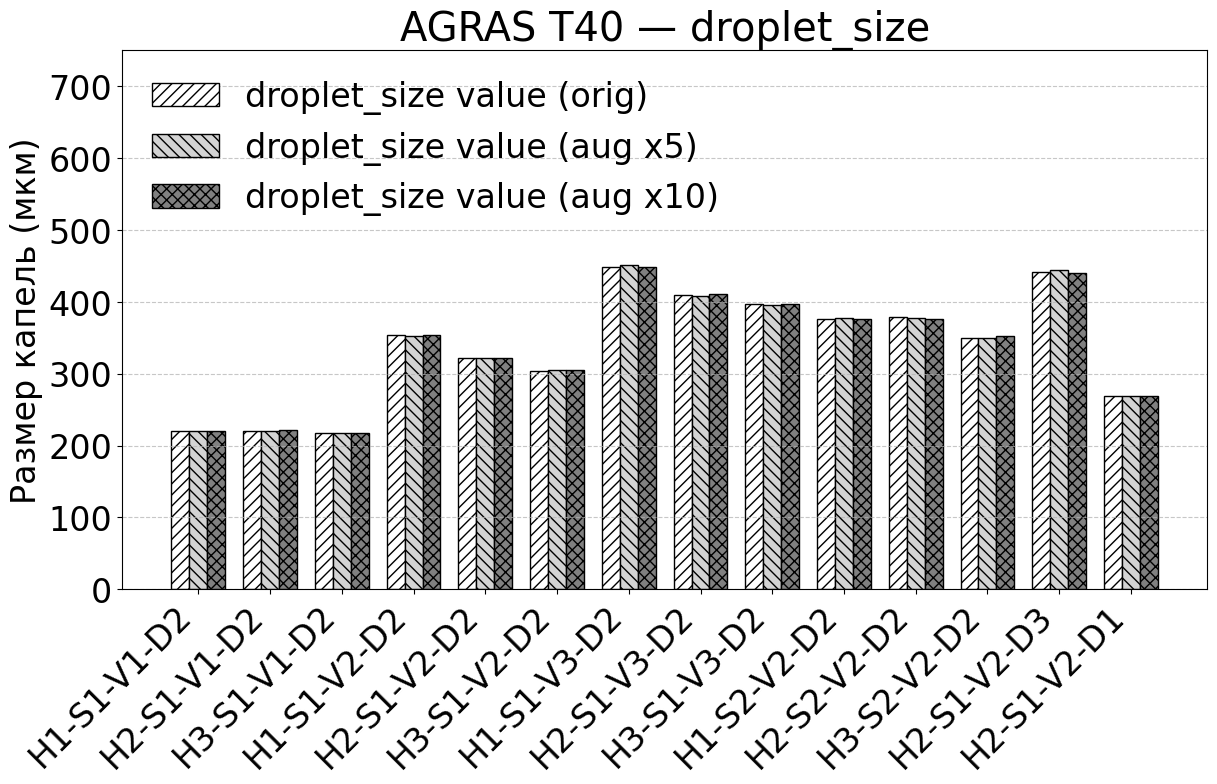
\includegraphics[width=.95\linewidth,valign=t]{my_folder/images/augment/spraying_performance/T40-droplet-size.png}
	\end{subfigure}
	\\[20pt]
	\adjustbox{minipage=1.3em,valign=t}{\subcaption{}\label{fig:augds-c}}%
	\begin{subfigure}[t]{\dimexpr.5\linewidth-1.3em\relax}
		\centering
		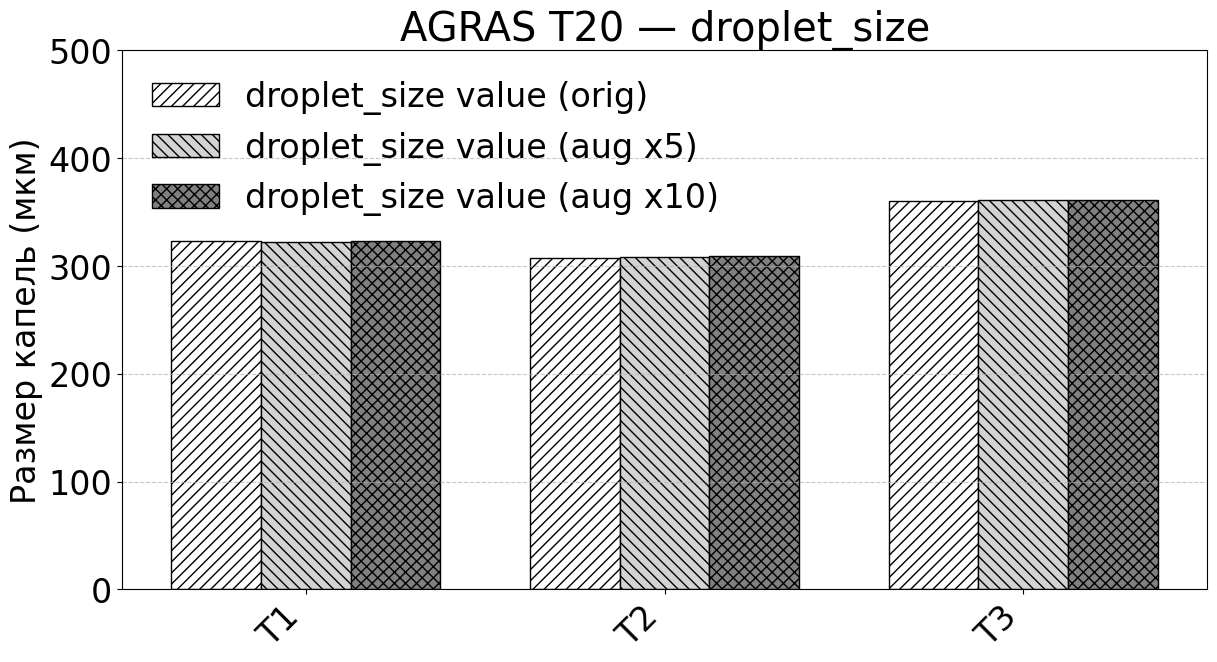
\includegraphics[width=.95\linewidth,valign=t]{my_folder/images/augment/droplet_deposition/T20-droplet-size.png}
	\end{subfigure}%
	\hfill %выровнять по ширине
	\adjustbox{minipage=1.3em,valign=t}{\subcaption{}\label{fig:augds-d}}%
	\begin{subfigure}[t]{\dimexpr.5\linewidth-1.3em\relax}
		\centering
		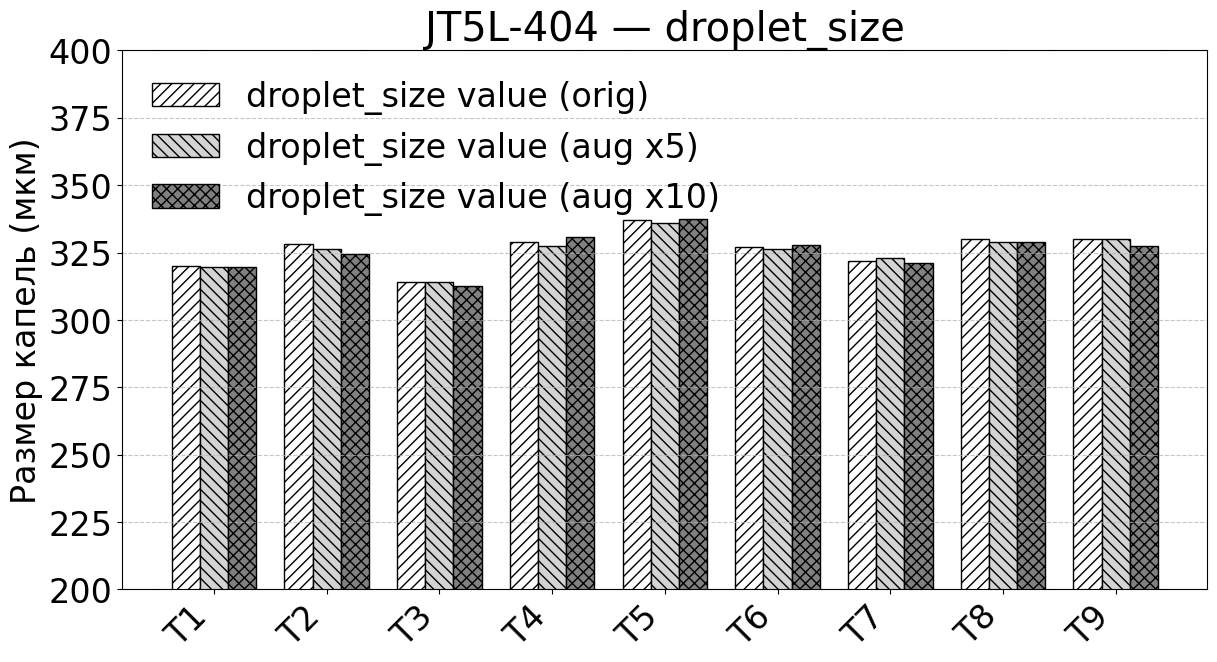
\includegraphics[width=.95\linewidth,valign=t]{my_folder/images/augment/coffee_science/JT5-droplet-size.png}
	\end{subfigure}
	\end{minipage}
	\captionsetup{justification=centering} %центрировать
	\caption{Распределение значений диаметра капель в исходной и аугментированных выборках: {\itshape a} --- AGRAS T30; {\itshape b} --- AGRAS T40; {\itshape c} --- AGRAS T20; {\itshape d} --- JT5L-404} 
	\label{fig:augment-droplet-size}
\end{figure}
\newpage

По графикам на рис. \ref{fig:augment-coverage} и \ref{fig:augment-droplet-size} видно, что аугментация экспериментальных данных в пятикратном и десятикратном объёме не приводит к существенным изменениям в распределении целевых переменных. Во всех наборах наблюдается высокая согласованность между средними значениями покрытия и диаметра капель в оригинальных и расширенных выборках: столбцы для «orig», «aug ×5» и «aug ×10» располагаются без выраженных смещений.

\section{Объединение и предварительная обработка данных} \label{ch2:proccessed}

После завершения аугментации данные из трёх расширенных датасетов были объединены в один общий. На этом этапе выполнялось выравнивание названий признаков путём, например, разбиения параметров погодных характеристик (температура, влажность, скорость ветра) на минимальные и максимальные значения. При объединении отсутствующие столбцы автоматически заполнялись пустыми значениями (NaN) для тех записей, в которых соответствующие измерения не проводились.

Дальнейший анализ показал, что многие признаки --- в основном связанные с морфологическими характеристиками растений и отдельными техническими параметрами БПЛА --- содержат пропуски в большей части строк, поскольку не во всех статьях приводился полный набор измерений. Для алгоритма CatBoost такая ситуация не требовала дополнительной обработки: пропуски оставлены, за исключением признака \texttt{experiment.params.atomization\_diameter}, где NaN заменены на значение \texttt{off}, отражающее отсутствие автоматизации у модели. Кроме того, столбец \texttt{experiment.name}, по результатам первоначального анализа, вносил сильную линейную зависимость между наблюдениями и целевыми переменными, поэтому он был удалён для исключения нежелательных корреляций.

В отличие от CatBoost, остальные алгоритмы не обладают встроенной поддержкой пропусков и требуют полного набора признаков. Поэтому все столбцы с хотя бы одним пустым значением были исключены, кроме тех, что непосредственно относятся к результатам эксперимента (значения покрытия и среднего диаметра капель), поскольку там пропуски означают лишь отсутствие измерений для одной из целевых метрик. После этого все оставшиеся категориальные признаки были преобразованы методом \texttt{one-hot encoding}, что позволило получить бинарные индикаторы для каждого уникального значения. Непрерывные числовые признаки затем подверглись масштабированию, улучшая сходимость линейной регрессии и регрессии опорных векторов.

\section{Выводы}

Аугментация в пяти- и десятикратном объёме не искажает распределения ключевых метрик, что подтверждено визуальными сравнениями. Объединение и очистка данных обеспечили единую структуру: для CatBoost сохранены все исходные признаки с NaN, для остальных ансамблей исключены колонки с пропусками и применено one-hot кодирование, а для MLR/SVR к этому добавлено масштабирование числовых признаков. Таким образом, были получены три полноценных набора данных, оптимизированных под требования соответствующих алгоритмов и готовых к оценке.